\documentclass{article}

\usepackage{fancyhdr}
\usepackage{extramarks}
\usepackage{amsmath}
\usepackage{amsthm}
\usepackage{amsfonts}
\usepackage{tikz}
\usepackage{listings}
%\usepackage[plain]{algorithm}
\usepackage{algpseudocode}
\usepackage{enumerate}
\usepackage{tikz}
\usepackage{xifthen}
\usepackage{xparse}
\usepackage{amsmath, amssymb}
\usepackage{lipsum}
\usepackage[lined,boxed,commentsnumbered]{algorithm2e}

\usetikzlibrary{automata,positioning}

%
% Basic Document Settings
%  

\topmargin=-0.45in
\evensidemargin=0in
\oddsidemargin=0in
\textwidth=6.5in
\textheight=9.0in
\headsep=0.25in

\linespread{1.1}

\pagestyle{fancy}
\lhead{\hmwkAuthorName}
\chead{\hmwkClass: \hmwkTitle}
\rhead{\firstxmark}
\lfoot{\lastxmark}
\cfoot{\thepage}

\renewcommand\headrulewidth{0.4pt}
\renewcommand\footrulewidth{0.4pt}

\setlength\parindent{0pt}

%
% Create Problem Sections
%

\newcommand{\enterProblemHeader}[1]{
    \nobreak\extramarks{}{Problem \arabic{#1} continued on next page\ldots}\nobreak{}
    \nobreak\extramarks{Problem \arabic{#1} (continued)}{Problem \arabic{#1} continued on next page\ldots}\nobreak{}
}

\newcommand{\exitProblemHeader}[1]{
    \nobreak\extramarks{Problem \arabic{#1} (continued)}{Problem \arabic{#1} continued on next page\ldots}\nobreak{}
    \stepcounter{#1}
    \nobreak\extramarks{Problem \arabic{#1}}{}\nobreak{}
}

\newcommand*\circled[1]{\tikz[baseline=(char.base)]{
		\node[shape=circle,draw,inner sep=2pt] (char) {#1};}}


\setcounter{secnumdepth}{0}
\newcounter{partCounter}
\newcounter{homeworkProblemCounter}
\setcounter{homeworkProblemCounter}{1}
\nobreak\extramarks{Problem \arabic{homeworkProblemCounter}}{}\nobreak{}

%
% Homework Problem Environment
%
% This environment takes an optional argument. When given, it will adjust the
% problem counter. This is useful for when the problems given for your
% assignment aren't sequential. See the last 3 problems of this template for an
% example.
%

\NewDocumentEnvironment{homeworkProblem}{s m}{
    \IfBooleanT{#1}{\newpage}
    \section{Problem \arabic{homeworkProblemCounter} {\small (#2)}}
    \setcounter{partCounter}{1}
    \enterProblemHeader{homeworkProblemCounter}

}{
    \exitProblemHeader{homeworkProblemCounter}
}

%
% Homework Details
%   - Title
%   - Due date
%   - Class
%   - Instructor
%   - Class number
%   - Name
%   - Student ID

\newcommand{\hmwkTitle}{Final Project}
\newcommand{\hmwkDueDate}{December 31, 2022}
\newcommand{\hmwkClass}{Probability and Mathematical Statistics}
\newcommand{\hmwkClassInstructor}{Professor Ziyu Shao}

%\newcommand{\hmwkClassID}{}

\newcommand{\hmwkAuthorName}{Ren Hui, Wanchen Su}
\newcommand{\hmwkAuthorID}{2021533089, 2021533067}

%
% Title Page
%

\title{
    \vspace{2in}
    \textmd{\textbf{\hmwkClass:\\  \hmwkTitle}}\\
    \normalsize\vspace{0.1in}\small{Due\ on\ \hmwkDueDate\ at 11:59am}\\
   %\vspace{2in}\Huge{\hmwkClassID}\\   
   \vspace{2in}
}

\author{
	Name: \textbf{\hmwkAuthorName} \\
	Student ID: \hmwkAuthorID}
\date{}


\renewcommand{\part}[1]{\textbf{\large Part (\alph{partCounter})}\stepcounter{partCounter}\\}

%
% Various Helper Commands
%

% Useful for algorithms
\newcommand{\alg}[1]{\textsc{\bfseries \footnotesize #1}}
% For derivatives
\newcommand{\deriv}[1]{\frac{\mathrm{d}}{\mathrm{d}x} (#1)}
% For partial derivatives
\newcommand{\pderiv}[2]{\frac{\partial}{\partial #1} (#2)}
% Integral dx
\newcommand{\dx}{\mathrm{d}x}
% Alias for the Solution section header
\newcommand{\solution}{\textbf{\Large Solution}}
% Probability commands: Expectation, Variance, Covariance, Bias
\newcommand{\E}{\mathrm{E}}
\newcommand{\Var}{\mathrm{Var}}
\newcommand{\Cov}{\mathrm{Cov}}
\newcommand{\Bias}{\mathrm{Bias}}

\begin{document}

\maketitle
\pagebreak

% Problem 1
\begin{homeworkProblem}{Part 1: classical Bandit Algorithms}
    \solution
    \begin{enumerate}
        \item[1,2.]
        See jupyter notebook.
        \item[3.]
        Accorrding to python simulation, the results are:\\
        \textbf{results for $\epsilon$-greedy:}\\
        \begin{tabular}[t]{|c|c|c|c|}
        \hline
         & $\epsilon$ = 0.1 & $\epsilon$ = 0.5 & $\epsilon$ = 0.9 \\
        \hline
        reward & 3415.895 & 3083.32 & 2748.985 \\
        \hline
        $\theta$ & $[0.699565\ 0.501675\ 0.398460]$ & $[0.700644\ 0.496887\ 0.398588]$ & $[0.700090\ 0.499850\ 0.398113]$ \\
        \hline
        \end{tabular}\\

        \textbf{results for UCB:}\\
        \begin{tabular}[t]{|c|c|c|c|}
        \hline
         & c = 0.1 & c = 0.5 & c = 0.9 \\
        \hline
        reward & 3410.44 & 2974.035 & 2824.62 \\
        \hline
        $\theta$ & $[0.700882\ 0.492749\ 0.384489]$ & $[0.700674\ 0.499007\ 0.398861]$ & $[0.701356\ 0.498778\ 0.400231]$ \\
        \hline
        \end{tabular}\\

        \textbf{results for TS:}\\
        \begin{tabular}[t]{|c|c|c|}
        \hline
         & a,b = [[1, 1], [1, 1], [1, 1]] & a,b = [[601, 401], [401, 601], [2, 3]]\\
        \hline
        reward & 3481.33 & 3490.945 \\
        \hline
        $\theta$ & $[0.6995964\ 0.45887541\ 0.37554019]$ & $[0.68296885\ 0.4001996\ 0.362563]$ \\
        \hline
        \end{tabular}\\

        \item[4.]
        Oracle value:$$E(r) = 5000\times0.7 = 3500$$
        \textbf{gap of $\epsilon$-greedy:}\\
        \begin{tabular}[t]{|c|c|c|c|}
        \hline
         & $\epsilon$ = 0.1 & $\epsilon$ = 0.5 & $\epsilon$ = 0.9 \\
        \hline
        reward & 3415.895 & 3083.32 & 2748.985 \\
        \hline
        gap & 84.105 & 416.68 & 751.015 \\
        \hline
        \end{tabular}\\

        \textbf{gap of UCB:}\\
        \begin{tabular}[t]{|c|c|c|c|}
        \hline
         & c = 0.1 & c = 0.5 & c = 0.9 \\
        \hline
        reward & 3410.44 & 2974.035 & 2824.62 \\
        \hline
        gap & 89.56 & 525.965 & 675.38 \\
        \hline
        \end{tabular}\\

        \textbf{gap of TS:}\\
        \begin{tabular}[t]{|c|c|c|}
        \hline
         & a,b = [[1, 1], [1, 1], [1, 1]] & a,b = [[601, 401], [401, 601], [2, 3]]\\
        \hline
        reward & 3481.33 & 3490.945 \\
        \hline
        gap & 18.67 & 9.905 \\
        \hline
        \end{tabular}\\

        As is shown above, with the given parameters, TS Algorithm is the best.\\
        
        In the $\epsilon$-greedy algorithm, $\epsilon$ decides the probability of choosing the max estimate of all the arms or choosing a random arm.
        Which means the larger $\epsilon$ is, the more evenly spread are the tests.\\
        In the UCB algorithm, the parameter c balances the estimation of $\theta_j$, and considers the number of trials on that arm.
        Increasing c means considering more about the number of test on that arm, which will alow the decision maker(DM) choose some of the less experimented arms.
        This helps in instances where the number of tests on a arm is quite small and therefore the $\theta$ of that arm is way less than it should be.\\
        If the initial value of $\alpha_j,\beta_j$ we passed in is too small,
        then the result of the first few tests may influence the final result greatly,
        and  only a few dozen tests are on the second and third arm. If this happens, the estimate value of $\theta$ will be rather inaccurate. 
        At the same time, the aggregated reward will be quite large because the DM spent very little time exploring.
        On the other hand, if the initial value of $\alpha_j,\beta_j$ we passed in is relativly large, this value of a and b may influence the final result greatly.
        As in the trial with parameter [[601, 401], [401, 601], [2, 3]], we can see that the final estimation of arm two is very close to $\frac{401}{401+601}$.
        In this case, the parameter we passed in is correct in which is the arm with the largest oracle value, so the aggregated reward is quite large.
        However, if the parameter passed in is contradictory to the actual oracle, it will take quite a long time to adjust. Consequently the aggregated reward is smaller.\\
        More impacts of $\epsilon$, c and $\alpha_j,\beta_j$ concerning exploration-exploitation will be disccussed in 5.
        \item[5.]
        In the case of all algorithms, more exploitation means that we choose to pull the arm that has the greatest current estimation more often. So if the estimate of each arm differs too much from the oracle value,
        or the arm we think yield the best probability is not really the best,
        after all tests, the total aggregated reward becomes smaller. More exploration means
        the estimated value of the reward of each arm is more accurate, it helps the decision maker choose the arm better, but the exploration means that the rewards during exploration could be less.\\
        For the $\epsilon$-greedy algorithm, the larger $\epsilon$ is, there is more chance of exploration than exploitation.
        So while $\epsilon$ grows, the gaps between the algorithm estimate and the oracle value decreases, but the sum of the reward of all trials is smaller because the DM spent too much time exploring when it is not that necessary.\\
        As for the UCB Algorithm, the exploration-exploitation trade-off depends on the value of c.
        Similar to the $\epsilon$-greedy algorithm, the larger c is, there is more exploration and less exploitation.
        As can be deduced from the data in the python simulation, for larger c, the estimated value for the third arm is more accurate.
        This means that there are more times when the decision maker choose arm c. Consequently, the aggregated rewards over N time slots are less.\\
        The TS Algorithm is rather different from the previous ones. Its exploration is based on the beta distribution. 
        In each round, the theta of each arm is generated by a beta distribution, with means of $\frac{a}{a+b}$. So there is a chance that an arm with large means will get a smaller theta in that round. This will result in exploration.
        But that probability is small, so arms with small oracle values may end up being pulled only a few times.
        Which makes the estimate value of arms 2 and 3 rather inaccurate. But the aggregated reward gained over the N trials should be the largest of all the algorithms.
        TS performs best in this case because the parameters a and b we passed in corresponds with the real oracle value. On the other hand, as the example in 5,
        if the parameters passed in is inaccurate, it could have a large influence on the aggregated reward. This is a default for having too little exploration.
        \item[6.]
        We mainly refered to \textsl{Multi-Armed Bandits with Correlated Arms} to improve the classical bandit algorithms.
        Before this, we also tried the method in \textsl{Multi-Armed Bandits with Dependent Arms}, which used clusters to proccess dependency, but its performance is not as good.
        So our final version is as below:
        \begin{enumerate}
            \item[a.] Data choice:
            After research, we found that the dependent multiarm bandit problem is often used in machine learning to decide which items to promote for each user.
            So besides using computer generated data to test our dependent bandit algorithm, we also used authentic data downloaded from the internet.
            We considered the real-life application of the dependent multi-arm bandit problem, more specifically, the problem of movie promotion.
            For app designers, they want to push book advertisments accorrding to user preference, and user preference is linked to certain traits of the user in question.
            We downloaded a dataset of viewer ratings on movies. The choice of movie we push for the viewer is the arm we choose, and the viewer's final rating is the reward.
            To match a three arm bandit machine, we implemented the dependent algorithm on choosing three movies to promote.
            \item[b.] Performance evaluation:
            To make the result more clear, we use expected regret ($E[Reg(T)]$) to analize the performance of our algorithm.
            The regret of an algorithm is defined as the difference between the cumulative reward of a genie policy, that always pulls the optimal arm, and the cumulative reward obtained by the algorithm over T rounds.
            So obviously its expectation in each round is the difference between the mean reward of the best arm and the mean reward of the choosen arm.
            We drew the cumulative regret of each round on a plot to visualize the performance of each algorithm.
            \item[c.] Dependency:
            After proccessing the data, we obtained pseudo-rewards, which provids an upper bound on the conditional expectation of a arm l given that we have recieved an reward r at another arm k.
            We use the defination of pseudo-rewards from the paper "Multi-Armed Bandits with Correlated Arms", which is: "Suppose we pull arm k and observe reward r, then the pseudo-reward of arm l with respect to arm k, denoted by $s_{l,k}(r)$, 
            is an upper bound on the conditional expected reward of arm l, i.e.,$$E[R_l|R_k = r]\leqslant s_{l,k}(r)$$ without loss of generality, we define $s_{l,l}(r)=r$."
            This information can be obtained in practice through either domain/expert knowledge or from controlled surveys. 
            Similarly, define $\phi_{l,k} = E[s_{l,k}(R_k)]$.
            \item[d.] Dependent bandit algorithm:
            We realized both the dependent UCB algorithm and the dependent TS algorithm. Since both is similar in principle, we will mainly disccuss the dependent UCB algorithm.\\
            The basic idea is to use dependency to eliminate some of the less competitive arms, so there are less choice each round, and the choices are closer to the best choice.\\
            \textbf{Step 1: Identify the set of significant arms} The set of significant arms at round t $S_t$ is defined to be the set of arms that have at least $t/arms$ samples.
            In other words, $S_t$ is the set of arms that have relativly large number of samples. So we will use the data of these arms to eliminate less competitive arms by dependency.\\
            \textbf{Step 2: Identify the set of competitive arms} First, find the largest estimated theta value so far by UCB(or TS) algorithm. Let that arm or the few arms that have the best theta be $C_t$ Then, for each arm l, find the smallest $\phi_{l,k}$ with $k\in S_t$.
            If this value is less than the largest estimated theta value so far, then this arm l is not competitive. Note that the $\phi$ value changes at each round so arm l is not eliminated forever.
            Denote the set of all competitive arms to be $A_t$\\
            \textbf{Step 3: Use bandit algorithm on $A_t\cup C_t$} Accorrding to the steps above, $A_t\cup C_t$ is the set of all competitive arms at round t.
        \end{enumerate}
        The specific algorithm we used is shown below.\\
        \begin{algorithm}[H]
            \SetAlgoLined
            Input: pseudo-rewards $s_{l,k}(r)$\\
            Initialize: $count[k] = 0, theta[k] = \infty$ for all k in arms\\
            \For {each round t}{
                Find $S_t$, the arm(s) that have been pulled significant times till the t-1 round.\\
                Define $k^{emp}(t) = argmax_{k\in S_t}\theta_k(t)$\\
                Initialize the competitive set $A_t$ as an empty set.\\
                \For {$k \in arms$}{
                    \If{$min_{l\in S_t}\phi_{k,l}(t)\geqslant \theta_{k^{emp}(t)}$}{
                        add arm k to $A_t$
                    }
                }
                Apply UCB to $A_t\cup {k^{emp}(t)}$\\
                Recieve reward and update reward, count[k], theta[k], pseudo-reward.
            }
            \caption{Dependent UCB}
          \end{algorithm}
          The following is the cumulative regret.\\
          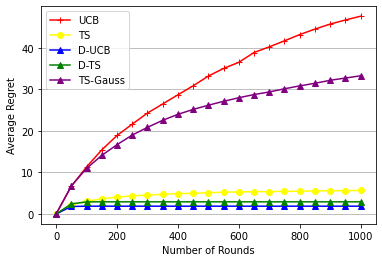
\includegraphics[width=0.5\textwidth]{part1.png}
        \item[*7.] reference reading:
        \begin{enumerate}[1]
            \item https://zhuanlan.zhihu.com/p/84140092, https://zhuanlan.zhihu.com/p/84200578, \\
            https://zhuanlan.zhihu.com/p/84338172
            \item Rahul Singh, Fang Liu, Yin Sun, Ness Shroff, \textsl{Multi-Armed Bandits with Dependent Arms}
            \item Samarth Gupta, Shreyas Chaudhari, Gauri Joshi, Osman Yağan, \textsl{Multi-Armed Bandits with Correlated Arms}
            \item S. Agrawal and N. Goyal, “Further optimal regret bounds for thompson sampling,” in \textsl{Artificial Intelligence and Statistics}, pp. 99-107, 2013.
        \end{enumerate}
    \end{enumerate}
\end{homeworkProblem}
\pagebreak

\begin{homeworkProblem}{Part 2: Bayesian Bandit Algorithms}
    \solution
    \begin{enumerate}
        \item[1.]
        See jupyter notebook for the simulation proccess. We simulated with the oracle value :\\
        \textbf{simulations:}\\
        \begin{tabular}[t]{|c|c|c|c|}
        \hline
        parameter & $\theta_1$ & $\theta_2$ & $\lambda$ \\
        \hline
        test 1 & 0.7 & 0.3 & 0.9 \\
        \hline
        test 2 & 0.4 & 0.5 & 0.9 \\
        \hline
        test 3 & 0.1 & 0.3 & 0.9 \\
        \hline
        \end{tabular}\\
        Let $r(n)$ be the reward over n pulls.
        \textbf{simulations:}\\
        \begin{tabular}[t]{|c|c|c|c|}
        \hline
        result & always choose best $E(r(25))$ & simulation $r(25)$ & always choose worst $E(r(n))$ \\
        \hline
        test 1 & 6.497471408615705 & 5.758137590942908 & 2.784630603692444 \\
        \hline
        test 2 & 4.641051006154074 & 4.247677424676706 & 3.71284080492326 \\
        \hline
        test 3 & 2.784630603692444 & 2.2136432344092114 & 0.928210201230815 \\
        \hline
        \end{tabular}\\
        \item[2.]
        If both $\theta_1$ and $\theta_2$ are relativly large, then we could end up with always pulling the first arm that succeeded.
        For example, if $\theta_1 = 0.8$, $\theta_2 = 0.9$, and the first arm we pulled is the first one, then there is a large possibility that the DM will always pull arm 1.
        We used 0.8 and 0.9 as the oracle value and asked the python simulation to print out the arm it chooses each time, and it shows clearly that it almost always sticks with the arm it chose in the first round.
        In fact, as it turns out, if the two arms have close possibility of giving a reward, this policy tend to behave not that well.
        \item[3.]
        Story proof:\\
        Let us be the decision maker(DM) of a two-armed bandit problem. Presume that the experiment lasts forever, 
        but the reward returned each time is reduced by multiplying $\lambda$, where $0<\lambda<1$. Put in mind that we as DM, 
        do not know the actual success probability of each arm. So let R($\alpha_1,\beta_1,\alpha_2,\beta_2$)represent the expected reward given the previous success and failures.
        So accorrding to LOTE, the expected reward of pulling the first arm is:
        $$R_1(\alpha_1,\beta_1) = P(success|\alpha_1,\beta_1)\times(\text{reward if succeed})+P(failure|\alpha_1,\beta_1)\times(\text{reward if failure})$$
        Which is:
        $$R_1(\alpha_1,\beta_1) = \frac{\alpha_1}{\alpha_1+\alpha_2}(1+\lambda R(\alpha_1+1,\beta_1,\alpha_2,\beta_2))+\frac{\alpha_2}{\alpha_1+\alpha_2}(\lambda R(\alpha_1,\beta_1+1,\alpha_2,\beta_2))$$
        $R_2$ is similar, the only difference is in the case of arm 2 we should change $\alpha_2$ and $\beta_2$ accorrdingly.
        Since we will always make the best desision at the moment, $R(\alpha_1,\beta_1,\alpha_2,\beta_2) = max{R_1(\alpha_1,\beta_1),R_2(\alpha_2,\beta_2)}$.
        Therefore, the given recurrence equation holds.
        \item[4.]
        The above recurrence equation can be solved by using dynamic programming in python simulation. We only need to type in the equation and manually set a ending condition,
        such as count the number of times it has been called repeatedly, and if it exceeds a certain $n$, then the function will return $\frac{\alpha}{\alpha+\beta}$.
        See jupyter notebook part2.ipynb for the simulation.
        \item[5.]
        The optimal policy will be to alter the algorithm in 4 slightly, so that after solving the equation with dynamic programming, we will get a 4d matrix, storing the corresponding decision we should make 
        with the known previous results. It should be noted that in this step, the case where either arm can be choosen must be threated with care. We denoted it as 0, rather than arm1 or 2, 
        and when the DM sees a 0 in the matirx it randomly chooses an arm to pull every trial. In this way the matix will not effect the DM more than it should.
        The DM will only need to check the matrix to know the arm it should choose. The simulation for the improved strategy is in part2.ipynb.
        The result is as below:
        \textbf{simulations:(results are averaged over 200 trials)}\\
        \begin{tabular}[t]{|c|c|c|c|}
        \hline
        test & actual theta & intuitive policy & Bayesian policy \\
        \hline
        test 1 & 0.8 0.3 & 6.526969462197445 & 6.768196035314434 \\
        \hline
        test 2 & 0.5 0.7 & 5.889886701348879 & 5.964659433792904 \\
        \hline
        test 3 & 0.7 0.9 & 7.719050567502581 & 7.767808893289861 \\
        \hline
        \end{tabular}\\
        Because of the influence of $\gamma$, the numeric result is not significant, so we used the regret analisys in part1 to show the performance more clearly.
        The below picture is the regret of the intuitive policy and the bayesian policy with actual theta at 0.7,0.9.\\
        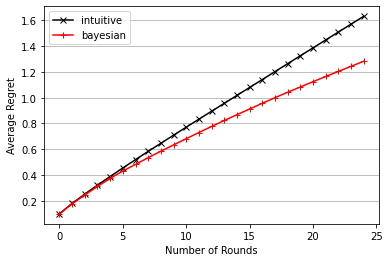
\includegraphics[width=0.5\textwidth]{part2.png}
        \item[*6.] reference reading:
        \begin{enumerate}[1]
            \item Richard S. Sutton and Andrew G. Barto, \textsl{Reinforcement Learning: An Introduction}
            \item Lucas Descause, \textsl{Reinforcement Learning with Function Approximation in Continuing Tasks: Discounted Return or Average Reward?}
        \end{enumerate}
    \end{enumerate}
\end{homeworkProblem}




\end{document}